% ------------------------------------------------------------------------------
% TYPO3 Version 10.2 - What's New (Italian Version)
%
% @license	Creative Commons BY-NC-SA 3.0
% @link		https://typo3.org/help/documentation/whats-new/
% @language	Italian
% ------------------------------------------------------------------------------

\section{Introduzione}
\begin{frame}[fragile]
	\frametitle{Introduzione}

	\begin{center}\huge{Introduzione}\end{center}
	\begin{center}\huge{\color{typo3darkgrey}\textbf{I fatti in breve}}\end{center}

\end{frame}

% ------------------------------------------------------------------------------
% TYPO3 Version 10.2 - The Facts

\begin{frame}[fragile]
	\frametitle{Introduzione}
	\framesubtitle{TYPO3 Versione 10.2 - I fatti in breve}

	\begin{itemize}
		\item Data di rilascio: 3 Dicembre 2019
		\item Tipo di rilascio: Sprint Release
	\end{itemize}

	\begin{figure}
		
\includegraphics[width=0.95\linewidth]{Introduction/typo3-v10-2-banner.png}
	\end{figure}

\end{frame}

% ------------------------------------------------------------------------------
% TYPO3 Version 10.2 - Executive Summary

\begin{frame}[fragile]
	\frametitle{Introduzione}
	\framesubtitle{Sintesi}

	\small
		La versione 10.2 di TYPO3 è la terza versione dello sprint per arrivare alla versione LTS
		(supporto a lungo termine) nel 2020. E' anche l'ultima versione dello sprint dell'anno.

		\vspace{0.2cm}

		Molte funzionalità sono state sviluppate durante la TYPO3 Initiative Week (T3INIT19)
		e TYPO3 v10.2 contiene già alcuni di questi sviluppi.

		\vspace{0.2cm}

		Questa versione apre la strada ad un ambiente all'avanguardia. TYPO3 v10.2 non supporta
		solo Symfony versione 5.0, ma è anche la prima versione di TYPO3 che supporta PHP
		versione 7.4. E' anche l'ultima versione prima della freeze release di febbraio 2020.

	\normalsize

\end{frame}

% ------------------------------------------------------------------------------
% System Requirements

\begin{frame}[fragile]
	\frametitle{Introduzione}
	\framesubtitle{Requisiti di sistema}

	\begin{itemize}
		\item PHP versione 7.2, 7.3 o 7.4
		\item Impostazioni PHP:

			\begin{itemize}
				\item \texttt{memory\_limit} >= 256M
				\item \texttt{max\_execution\_time} >= 240s
				\item \texttt{max\_input\_vars} >= 1500
				\item l'opzione di compilazione \texttt{-}\texttt{-disable-ipv6} \underline{non} deve essere usata
			\end{itemize}

		\item La maggior parte dei database supportati da \textbf{Doctrine DBAL} funzionano anche con TYPO3.
			I DB verificati sono ad esempio:
	\end{itemize}

	\begin{figure}
		
\includegraphics[width=0.80\linewidth]{Introduction/logo-databases.png}
	\end{figure}

\end{frame}

% ------------------------------------------------------------------------------
% Development, Release and Maintenance Timeline

\begin{frame}[fragile]
	\frametitle{Introduzione}
	\framesubtitle{Sviluppo, tempi di rilascio e mantenimento}

	\textbf{TYPO3 v10}

	\begin{figure}
		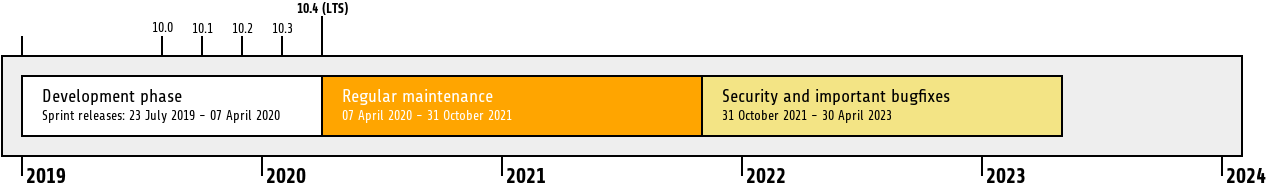
\includegraphics[width=1\linewidth]{Introduction/typo3-v10-lifecycle.png}
	\end{figure}

	\textbf{Supporto esteso}\newline
	\smaller
		La \href{https://typo3.com}{TYPO3 GmbH} offre ulteriori opzioni di supporto
		per TYPO3 v10 LTS anche dopo il 30 Aprile 2023, per ulteriori due anni.
	\normalsize

\end{frame}

% ------------------------------------------------------------------------------
% TYPO3 v10 Roadmap

\begin{frame}[fragile]
	\frametitle{Introduction}
	\framesubtitle{TYPO3 v10 Roadmap}

	Date di rilascio e loro obiettivi principali:

	\begin{itemize}

		\item v10.0 \tabto{1.1cm}23/Lug/2019\tabto{3.4cm}Preparare la strada per nuovi concetti e API entusiasmanti
		\item v10.1 \tabto{1.1cm}01/Ott/2019\tabto{3.4cm}Miglioramenti nel routing e nel gestore di sito v2
		\item
			\begingroup
				\color{typo3orange}
				v10.2 \tabto{1.1cm}03/Dic/2019\tabto{3.4cm}Miglioramenti al motore di rendering Fluid
			\endgroup
		\item v10.3 \tabto{1.1cm}04/Feb/2020\tabto{3.4cm}Conferma della funzionalità
		\item v10.4 \tabto{1.1cm}07/Apr/2020\tabto{3.4cm}Rilascio LTS (Long-term Support)

	\end{itemize}

	\smaller
		\url{https://typo3.org/article/typo3-v10-roadmap/}\newline
		\url{https://typo3.org/article/typo3-v10-safe-and-sound/}
	\normalsize

\end{frame}

% ------------------------------------------------------------------------------
% Installation

\begin{frame}[fragile]
	\frametitle{Introduzione}
	\framesubtitle{Installazione}

	\begin{itemize}
		\item Procedura ufficiale, \textit{classica}, di installazione in Linux/Mac OS X\newline
			(Directory Root ad esempio \texttt{/var/www/site/htdocs}):
\begin{lstlisting}
$ cd /var/www/site
$ wget --content-disposition get.typo3.org/10.2
$ tar xzf typo3_src-10.2.0.tar.gz
$ cd htdocs
$ ln -s ../typo3_src-10.2.0 typo3_src
$ ln -s typo3_src/index.php
$ ln -s typo3_src/typo3
$ touch FIRST_INSTALL
\end{lstlisting}

		\item Link simbolici in Microsoft Windows:

			\begin{itemize}
				\item Usa \texttt{junction} in Windows XP/2000
				\item Usa \texttt{mklink} in Windows Vista e Windows 7 e superiori
			\end{itemize}

	\end{itemize}
\end{frame}

% ------------------------------------------------------------------------------
% Installation using composer

\begin{frame}[fragile]
	\frametitle{Installazione e aggiornamento}
	\framesubtitle{Installazione con \texttt{composer}}

	\begin{itemize}
		\item Installazione con \textit{composer} in Linux, Mac OS X e Windows 10:
\begin{lstlisting}
$ cd /var/www/site/
$ composer create-project typo3/cms-base-distribution typo3v10 ^10.2
\end{lstlisting}

		\item In alternativa, create il vostro file \texttt{composer.json} ed eseguite:
\begin{lstlisting}
$ composer install
\end{lstlisting}

			Maggiori informazioni e un esempio di file \texttt{composer.json} sono disponibili su:\newline
			\smaller
				\href{https://composer.typo3.org}{https://composer.typo3.org}
			\normalsize

	\end{itemize}
\end{frame}

% ------------------------------------------------------------------------------
